\section{Proposed RAVM-DT Algorithm}
\label{sec:method}

\subsection{Overview}
RAVM-DT solves the decision problem in Section~\ref{sec:problem} by separating candidate adaptation from deployment commitment. At stage $t$, update data produce one candidate state, recent and bounded historical verification evidence compare that candidate with the current deployed state, and a selective decision either commits the candidate or retains the current state. Current verification data enter the historical buffer only after the decision. Figure~\ref{fig:overview} summarizes this workflow.

\begin{figure}[t]
\centering
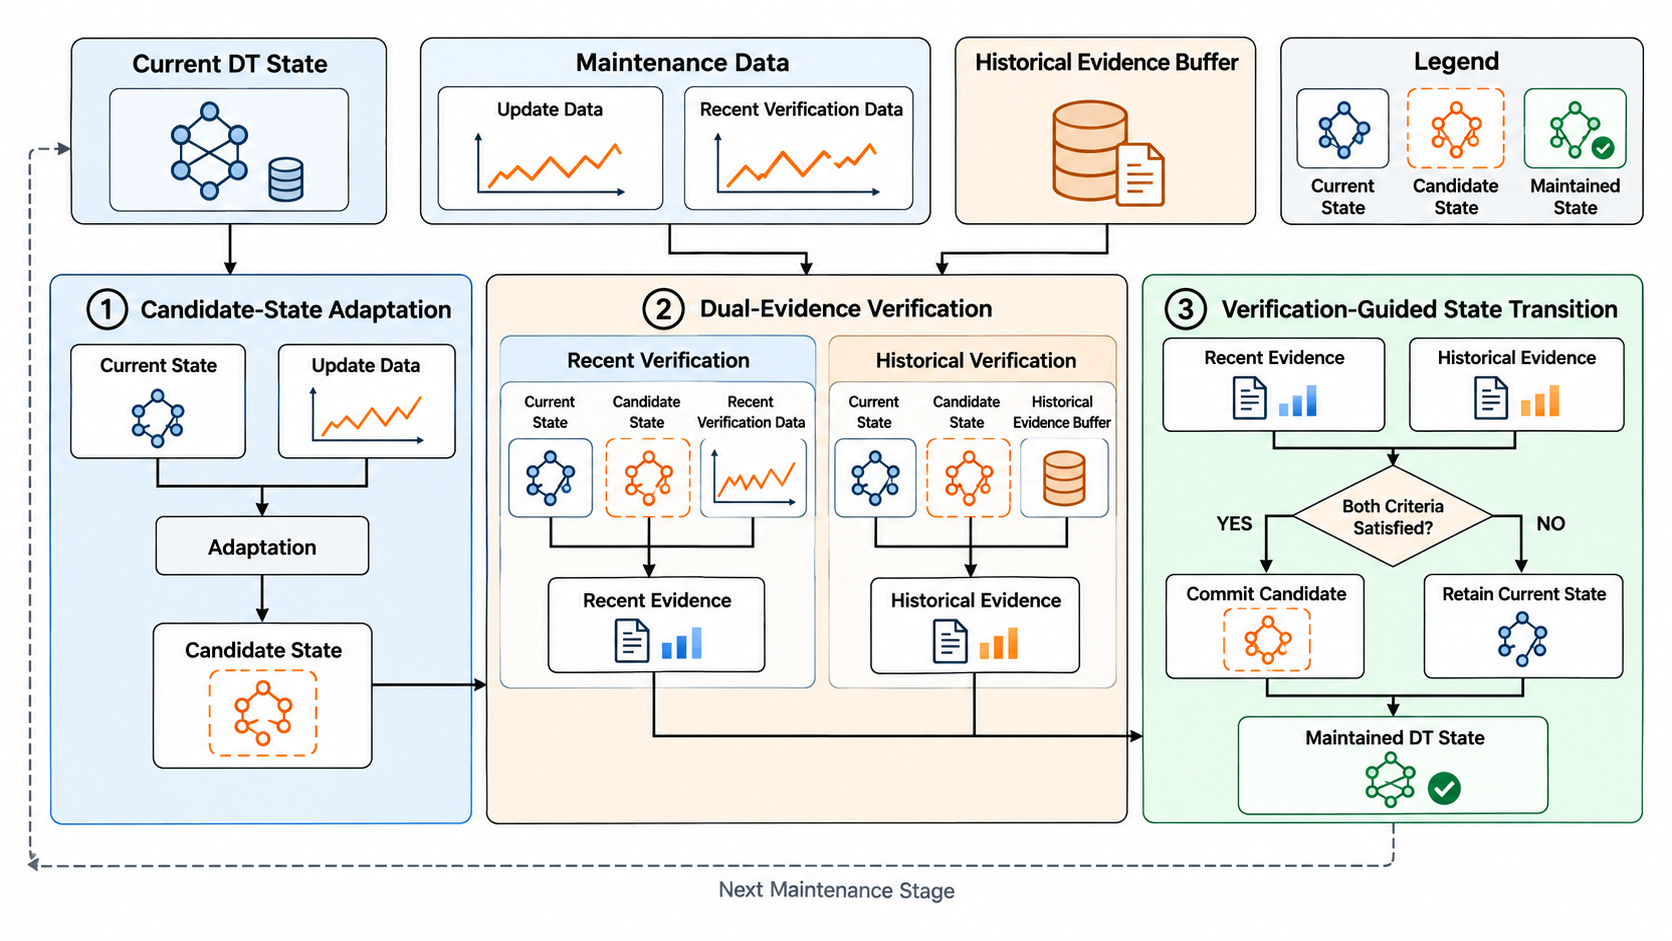
\includegraphics[width=0.92\textwidth]{fig2_ravm_dt_framework.pdf}
\caption{Overview of RAVM-DT. A single candidate state is adapted from the current DT state using update data, evaluated through recent and bounded historical evidence, and committed only when both criteria support replacement; otherwise, the current state is retained as the maintained DT state.}
\label{fig:overview}
\end{figure}

\subsection{Candidate-State Adaptation}
At each stage, the candidate starts as an isolated copy of the current deployed state and is optimized only with update data. Let $\mathcal B^{(s)}_{c,t}\subseteq\mathcal D^{\mathrm{upd}}_{c,t}$ denote the update mini-batch used at step $s$. A gradient-based realization of the candidate-adaptation operator in Eq.~\eqref{eq:candidate} is
\begin{equation}
\begin{aligned}
\theta^{(0)}_{c,t}&=\theta_{c,t-1},\\
\theta^{(s+1)}_{c,t}&=\theta^{(s)}_{c,t}-\eta\nabla_{\theta}\mathcal L\!\left(\mathcal B^{(s)}_{c,t};(a_c,\theta^{(s)}_{c,t})\right),\quad s=0,\ldots,S-1,\\
\widetilde{\theta}_{c,t}&=\theta^{(S)}_{c,t},\qquad \widetilde M_{c,t}=(a_c,\widetilde{\theta}_{c,t}),
\end{aligned}
\label{eq:adaptation}
\end{equation}
where $S$ is the stage-level adaptation budget and $\eta$ the learning rate. The complete update subset defines the sampling pool, while $\mathcal D^{\mathrm{ver}}_{c,t}$ is excluded from parameter updates and the deployed state is unchanged until commitment.

\subsection{Dual-Evidence Verification}
Each verification collection is partitioned chronologically into $B$ block units; target windows belong to one block, although their input contexts may overlap because of sliding-window construction. Let $\mathcal E^{\mathrm{rec}}_{c,t}=\mathcal D^{\mathrm{ver}}_{c,t}$ and let $\mathcal E^{\mathrm{hist}}_{c,t-1}$ denote blocks retained in a bounded historical buffer. Before the first online stage, $\mathcal H_{c,0}$ is initialized from target-specific pre-maintenance verification evidence. For $q\in\{\mathrm{rec},\mathrm{hist}\}$ and chronological block $\mathcal E^{q}_{c,t,j}$, RAVM-DT evaluates the candidate and current state on the same block:
\begin{equation}
d^{q}_{c,t,j}=\mathcal L\!\left(\mathcal E^{q}_{c,t,j};\widetilde M_{c,t}\right)-\mathcal L\!\left(\mathcal E^{q}_{c,t,j};M_{c,t-1}\right).
\label{eq:paired}
\end{equation}
Negative values favor the candidate. The paired differences are summarized by
\begin{equation}
\begin{aligned}
m^{q}_{c,t}&=\operatorname{median}_{j}d^{q}_{c,t,j},\\
r^{q}_{c,t}&=\operatorname{median}_{j}\left|d^{q}_{c,t,j}-m^{q}_{c,t}\right|,\\
U^{q}_{c,t}&=m^{q}_{c,t}+\kappa_q r^{q}_{c,t},\qquad q\in\{\mathrm{rec},\mathrm{hist}\},
\end{aligned}
\label{eq:evidence-score}
\end{equation}
where $\kappa_q\geq0$ controls the penalty for disagreement among verification blocks. $U^{q}_{c,t}$ is a robust conservative evidence score, not a formal statistical confidence bound.

\subsection{Verification-Guided State Transition}
Let $\delta_{\mathrm{imp}}\geq0$ be the required recent improvement and $\delta_{\mathrm{ret}}\geq0$ the tolerated historical degradation. The deployment decision is
\begin{equation}
u_{c,t}=\begin{cases}
1, & U^{\mathrm{rec}}_{c,t}\leq-\delta_{\mathrm{imp}}\ \text{and}\ U^{\mathrm{hist}}_{c,t}\leq\delta_{\mathrm{ret}},\\
0, & \text{otherwise}.
\end{cases}
\label{eq:commit-rule}
\end{equation}
Thus, recent evidence requires adaptation benefit while historical evidence limits degradation of recently retained behavior. The historical buffer has capacity $C_{\mathrm{hist}}$; after the stage-$t$ decision, current verification blocks are appended and the oldest blocks are evicted if necessary. This ordering prevents current verification data from influencing their own decision through the historical branch and limits the effect of obsolete regimes.

\begin{Algorithm}[RAVM-DT Maintenance for Center $c$ at Stage $t$]
\label{alg:method}
\normalfont\small
\setlength{\emergencystretch}{1.5em}
\begin{enumerate}[label=\arabic*.,leftmargin=2.2em,labelwidth=1.2em,labelsep=0.4em,itemsep=0pt,topsep=1pt]
\item \textbf{Input:} $M_{c,t-1}$, $\mathcal D^{\mathrm{upd}}_{c,t}$, $\mathcal D^{\mathrm{ver}}_{c,t}$, historical buffer $\mathcal H_{c,t-1}$, and method parameters.
\item Adapt on $\mathcal D^{\mathrm{upd}}_{c,t}$ using Eq.~\eqref{eq:adaptation} to obtain $\widetilde M_{c,t}$.
\item Form recent and historical evidence and compute Eqs.~\eqref{eq:paired}--\eqref{eq:evidence-score}.
\item Determine $u_{c,t}$ by Eq.~\eqref{eq:commit-rule} and update $M_{c,t}$ by Eq.~\eqref{eq:commit-state}.
\item \textbf{After the decision}, append current verification blocks to $\mathcal H_{c,t-1}$ and evict the oldest blocks if required.
\item \textbf{Return:} $M_{c,t}$ and the updated buffer $\mathcal H_{c,t}$.
\end{enumerate}
\end{Algorithm}

\subsection{Decision-Parameter Calibration}
Let $\gamma\in\Gamma$ denote a candidate decision-parameter configuration. On calibration data disjoint from final evaluation, let $\widehat{\mathcal R}(\gamma)$, $\widehat{\mathcal H}(\gamma)$, and $\widehat{\mathcal S}(\gamma)$ denote empirical lifecycle loss, harmful-transition frequency, and harmful-transition downside. We select
\begin{equation}
\gamma^{*}\in\arg\min_{\gamma\in\Gamma}\widehat{\mathcal R}(\gamma)
\quad\mathrm{s.t.}\quad
\widehat{\mathcal H}(\gamma)\leq\rho,\qquad
\widehat{\mathcal S}(\gamma)\leq\epsilon.
\label{eq:calibration}
\end{equation}
The selected configuration is fixed before final evaluation. Equation~\eqref{eq:calibration} is an offline calibration rule; online decisions still use only information available before the subsequent service interval.
